\documentclass[tikz,border=8pt]{standalone}
\usepackage{amsmath,amssymb}
\usetikzlibrary{arrows.meta,calc,decorations.markings,shapes.geometric}

\begin{document}
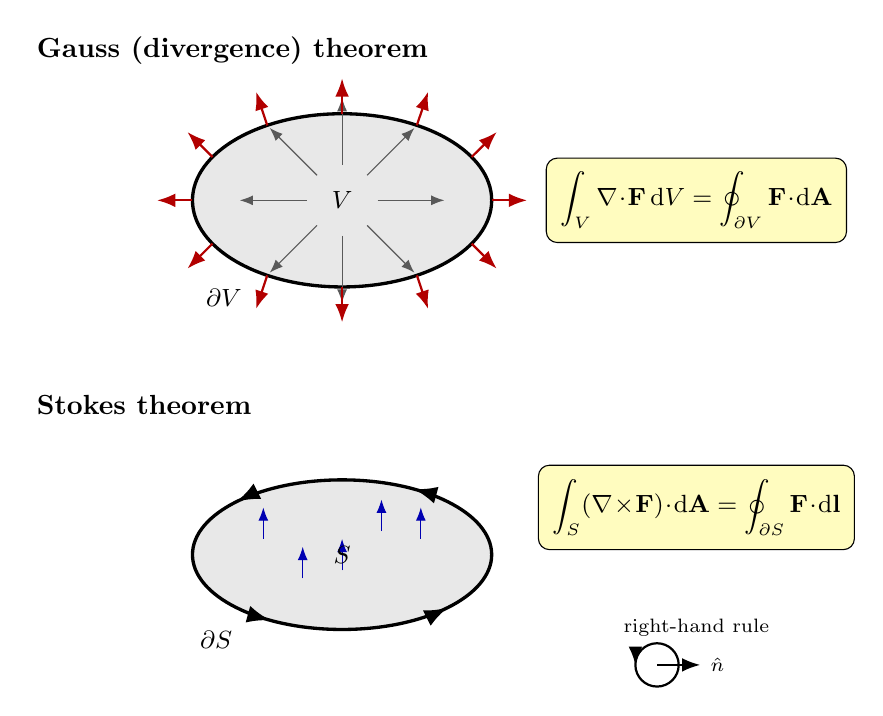
\begin{tikzpicture}[>=Latex]

  % TOP — divergence theorem
  \begin{scope}[yshift=4.5cm]
    \node[font=\bfseries, anchor=west] at (-5.5, 1.9) {Gauss (divergence) theorem};

    \begin{scope}[xshift=-1.5cm]
      \fill[gray!18] (0,0) ellipse (1.9 and 1.1);
      \draw[very thick] (0,0) ellipse (1.9 and 1.1);
      % interior arrows
      \foreach \angle in {0,45,90,135,180,225,270,315}{
        \draw[->, gray!70!black] (\angle:0.45) -- (\angle:1.3);
      }
      % outward flux arrows on boundary
      \foreach \angle in {0,30,60,90,120,150,180,210,240,270,300,330}{
        \pgfmathsetmacro{\rx}{1.9*cos(\angle)}
        \pgfmathsetmacro{\ry}{1.1*sin(\angle)}
        \pgfmathsetmacro{\enx}{cos(\angle)/1.9}
        \pgfmathsetmacro{\eny}{sin(\angle)/1.1}
        \pgfmathsetmacro{\nrm}{sqrt(\enx*\enx + \eny*\eny)}
        \pgfmathsetmacro{\dx}{0.45*\enx/\nrm}
        \pgfmathsetmacro{\dy}{0.45*\eny/\nrm}
        \draw[->, red!70!black, thick] (\rx,\ry) -- ++ (\dx, \dy);
      }
      \node[font=\small] at (0, 0) {$V$};
      \node[anchor=north, font=\small] at (-1.5, -1.0) {$\partial V$};
    \end{scope}

    \node[align=left, font=\small, fill=yellow!25, draw, rounded corners, inner sep=5pt]
      at (3.0, 0) {$\displaystyle\int_V\nabla\!\cdot\!\mathbf F\,\mathrm dV=\oint_{\partial V}\mathbf F\!\cdot\!\mathrm d\mathbf A$};
  \end{scope}

  % BOTTOM — Stokes theorem
  \begin{scope}[yshift=0cm]
    \node[font=\bfseries, anchor=west] at (-5.5, 1.9) {Stokes theorem};

    \begin{scope}[xshift=-1.5cm]
      \fill[gray!18] (0,0) ellipse (1.9 and 0.95);
      \draw[very thick, postaction={decorate, decoration={markings,
        mark=at position 0.15 with {\arrow{>}},
        mark=at position 0.40 with {\arrow{>}},
        mark=at position 0.65 with {\arrow{>}},
        mark=at position 0.90 with {\arrow{>}}}}] (0,0) ellipse (1.9 and 0.95);

      % curl normal arrows
      \draw[->, blue!70!black] (-1.0,  0.2) -- ++ (0, 0.4);
      \draw[->, blue!70!black] ( 0.0, -0.2) -- ++ (0, 0.4);
      \draw[->, blue!70!black] ( 1.0,  0.2) -- ++ (0, 0.4);
      \draw[->, blue!70!black] (-0.5, -0.3) -- ++ (0, 0.4);
      \draw[->, blue!70!black] ( 0.5,  0.3) -- ++ (0, 0.4);

      \node[font=\small] at (0.0, 0.0) {$S$};
      \node[anchor=north, font=\small] at (-1.6, -0.85) {$\partial S$};
    \end{scope}

    % right-hand-rule inset
    \begin{scope}[xshift=2.5cm, yshift=-1.4cm, scale=0.55]
      \draw[->, thick] (0,0) -- (1.0, 0) node[right, font=\scriptsize]{$\hat n$};
      \draw[->, thick, postaction={decorate, decoration={markings,
        mark=at position 0.5 with {\arrow{>}}}}] (0,0) circle (0.5);
      \node[font=\scriptsize, anchor=west] at (-1.0, 0.85) {right-hand rule};
    \end{scope}

    \node[align=left, font=\small, fill=yellow!25, draw, rounded corners, inner sep=5pt]
      at (3.0, 0.6) {$\displaystyle\int_S(\nabla\!\times\!\mathbf F)\!\cdot\!\mathrm d\mathbf A=\oint_{\partial S}\mathbf F\!\cdot\!\mathrm d\mathbf l$};
  \end{scope}
\end{tikzpicture}
\end{document}
